%%%%%%%%%%%%%%%%%%%%%%%%%%%%%
% Standard header for working papers
%
% WPHeader.tex
%
%%%%%%%%%%%%%%%%%%%%%%%%%%%%%

\documentclass[11pt]{article}

%%%%%%%%%%%%%%%%%%%%
%% Include general header where common packages are defined
%%%%%%%%%%%%%%%%%%%%



%%%%%%%%%%%%%%%%%%%%%%%%%%
%% TEMPLATES
%%%%%%%%%%%%%%%%%%%%%%%%%%


% Simple Tabular

%\begin{tabular}{ |c|c|c| } 
% \hline
% cell1 & cell2 & cell3 \\ 
% cell4 & cell5 & cell6 \\ 
% cell7 & cell8 & cell9 \\ 
% \hline
%\end{tabular}





%%%%%%%%%%%%%%%%%%%%%%%%%%
%% Packages
%%%%%%%%%%%%%%%%%%%%%%%%%%



% encoding 
\usepackage[utf8]{inputenc}
%\usepackage[T1]{fontenc}
\usepackage{ctex}

% general packages without options
\usepackage{amsmath,amssymb,amsthm,bbm}

% graphics
\usepackage{graphicx,transparent,eso-pic}

% text formatting
\usepackage[document]{ragged2e}
\usepackage{pagecolor,color}
%\usepackage{ulem}
\usepackage{soul}







%%%%%%%%%%%%%%%%%%%%%%%%%%
%% Maths environment
%%%%%%%%%%%%%%%%%%%%%%%%%%

%\newtheorem{theorem}{Theorem}[section]
%\newtheorem{lemma}[theorem]{Lemma}
%\newtheorem{proposition}[theorem]{Proposition}
%\newtheorem{corollary}[theorem]{Corollary}

%\newenvironment{proof}[1][Proof]{\begin{trivlist}
%\item[\hskip \labelsep {\bfseries #1}]}{\end{trivlist}}
%\newenvironment{definition}[1][Definition]{\begin{trivlist}
%\item[\hskip \labelsep {\bfseries #1}]}{\end{trivlist}}
%\newenvironment{example}[1][Example]{\begin{trivlist}
%\item[\hskip \labelsep {\bfseries #1}]}{\end{trivlist}}
%\newenvironment{remark}[1][Remark]{\begin{trivlist}
%\item[\hskip \labelsep {\bfseries #1}]}{\end{trivlist}}

%\newcommand{\qed}{\nobreak \ifvmode \relax \else
%      \ifdim\lastskip<1.5em \hskip-\lastskip
%      \hskip1.5em plus0em minus0.5em \fi \nobreak
%      \vrule height0.75em width0.5em depth0.25em\fi}



%%%%%%%%%%%%%%%%%%%%
%% Idem general commands
%%%%%%%%%%%%%%%%%%%%
%% Commands

\newcommand{\noun}[1]{\textsc{#1}}


%% Math

% Operators
\DeclareMathOperator{\Cov}{Cov}
\DeclareMathOperator{\Var}{Var}
\DeclareMathOperator{\E}{\mathbb{E}}
\DeclareMathOperator{\Proba}{\mathbb{P}}

\newcommand{\Covb}[2]{\ensuremath{\Cov\!\left[#1,#2\right]}}
\newcommand{\Eb}[1]{\ensuremath{\E\!\left[#1\right]}}
\newcommand{\Pb}[1]{\ensuremath{\Proba\!\left[#1\right]}}
\newcommand{\Varb}[1]{\ensuremath{\Var\!\left[#1\right]}}

% norm
\newcommand{\norm}[1]{\left\lVert #1 \right\rVert}



% argmin
\DeclareMathOperator*{\argmin}{\arg\!\min}


% amsthm environments
\newtheorem{definition}{Definition}
\newtheorem{proposition}{Proposition}
\newtheorem{assumption}{Assumption}

%% graphics

% renew graphics command for relative path providment only ?
%\renewcommand{\includegraphics[]{}}





\renewcommand{\abstractname}{Abstract}
\renewcommand\refname{References}
\renewcommand\figurename{Figure}

% comments and responses
\usepackage{xparse}
\usepackage{ifthen}
\DeclareDocumentCommand{\comment}{m o o o o}
{\ifthenelse{\draft=1}{
    \textcolor{red}{\textbf{C : }#1}
    \IfValueT{#2}{\textcolor{blue}{\textbf{A1 : }#2}}
    \IfValueT{#3}{\textcolor{ForestGreen}{\textbf{A2 : }#3}}
    \IfValueT{#4}{\textcolor{red!50!blue}{\textbf{A3 : }#4}}
    \IfValueT{#5}{\textcolor{Aquamarine}{\textbf{A4 : }#5}}
 }{}
}


% todo
\newcommand{\todo}[1]{
\ifthenelse{\draft=1}{\textcolor{red!50!blue}{\textbf{TODO : \textit{#1}}}}{}
}


%\usepackage[UTF8]{ctex}



% geometry
\usepackage[margin=2cm]{geometry}

% layout : use fancyhdr package
\usepackage{fancyhdr}
\pagestyle{fancy}

\makeatletter

\renewcommand{\headrulewidth}{0.4pt}
\renewcommand{\footrulewidth}{0.4pt}
\fancyhead[RO,RE]{\textit{Working Paper}}
\fancyhead[LO,LE]{G{\'e}ographie-Cit{\'e}s}
\fancyfoot[RO,RE] {\thepage}
\fancyfoot[LO,LE] {\noun{C. Losavio and J. Raimbault}}
\fancyfoot[CO,CE] {}

\makeatother


%%%%%%%%%%%%%%%%%%%%%
%% Begin doc
%%%%%%%%%%%%%%%%%%%%%

\begin{document}






%%%%%
% variable to include comments or not in the compilation ; set to 1 to include
\def \draft {1}
%\def \draft {0}



\title{Agent-based Modeling of Migrant Workers Residential Dynamics within a Mega-city Region: the Case of Pearl River Delta, China
%Challenging Preconceived Ideas with an Agent-based Model
\bigskip\\
\textit{Working Paper}
}
\author{\noun{Cinzia Losavio} and \noun{Juste Raimbault}\\
UMR CNRS 8504 Géographie-cités
}
\date{}




\maketitle

\justify


\begin{abstract}
Over the last three decades, rural-urban migrant-workers have been a driving force for China's economy, raising attention on associated socio-economical issues. However, the importance of their economic diversity and social mobility has been poorly considered in the analysis of urban development strategy.
We use an agent-based model to simulate residential dynamics of migrants in Pearl River Delta (PRD) mega city region, taking into account the full range of migrants’ socio-economical status and their evolution. Mega-city regions have become a new scale of Chinese State regulation, and PRD represent the most prosperous and dynamic one in term of migration waves, standing as an ideal unit of analysis.
Our model unveils emergent patterns of dynamics, from micro behavior rules of discrete mobility choices. These choices are conditional to urban and economic environment, which evolution is controlled by meso-scale independent dynamics.
The two scales are coupled through the dependence of discrete choice utilities to generalized accessibility that combines patch-level urban and economic context with a feedback of the dynamics themselves. This multi-scale aspect is crucial to distinguish endogenous form exogenous effects in regional migration patterns.
We perform simulations to internally validate the model on synthetic data, by assessing statistical consistence and establishing phase diagrams across the parameter space.
The application to the case study allows first to test how variation in socio-economic status yield more complex trajectories, and secondly to identify how the Party-State persist in controlling internal migration flows in a more sophisticated and strategically redefined way.
Further work is directed towards a qualitative external validation of the model, by calibrating free parameters to reproduce meso-scale stylized facts, in order to guide interpretations of emergent outputs and potential policy applications.

\bigskip

\noindent\textbf{Keywords : } \textit{Mingong ; Residential Dynamics ; Agent-based Modeling ; Zhuijiang Delta Mega-city Region}
\end{abstract}




%%%%%%%%%%%%%%%%%%%%
\section{Introduction}


%%%%%%%%%%%%%%%%%%%%
\subsection{Context}

\paragraph{Mega-city Regions}

Mega-city regions (MCRs) are integrated sets of cities and their surrounding suburban hinterlands across which labour and capital can be reallocated at very low cost~\cite{florida2008rise}. It was first coined by Gottmann~\cite{gottman1961megalopolis} using the term megalopolis, that he defines as “urban area of several tens of millions of people, including several cities and major urban centers, and extending continuously over several 100 km”. It represents the new economic unit that emerges as metropolitan regions not only grow upward and become denser but also grow outward and into one another. These spaces result of the networking of a group of metropolitan areas deployed around very large cities and it is characterized by the “symbiosis between urban and rural areas”. Other characteristic are migration flows, density of connections, and regional migration patterns. 



\paragraph{Pearl River Delta}

Since the gradual decentralization of the state power which occurred in the beginning of  1990 Mega-city regions have become a new scale of Chinese State regulation, and in particular the pearl River Delta, represent the most prosperous and dynamic one in term of migration waves. That’s why we choose PRD as our unit of study. Since the Open Door Policy was implemented in 1978 the PRD launch a process of rapid economic and social transformation, becoming a global manufacturing region attracting an increasing number of migrant-workers from all over China. In fact, PRD was designed as an open economic zone in 1984, and was granted many ‘one step ahead’ policies to attract foreign capital, becoming the most important exporter center since economic reform. That results in an astonishing rise of population in the area. That today count more than 50 million people. If during the first year of the opening-up reforms the barycenter of the region was Guangzhou, over the last decade PRD has become increasing polycentric.
Taking PRD as the unit of our model we try to reproduce migrants residential patterns taking into account the full range of migrants’ socio-economical status and their evolution. 



\paragraph{Migrant Workers in PRD}


Even though migrants workers are generally considered and treated as a uniform category, my previous research showed how considering their economical, cultural and human capital migrants workers are a very diversified social category. Especially 3 dimension are fundamental to understand migrant workers:
\begin{itemize}
\item Professional Dimension : industry, construction, private sector, services (will change not only their economical situation but which influence  migrants’ trajectory and the staying duration in the city and their residential choice.
\item Residential Dimension : We could recognize two under-categories, with different socio-economic situation: (i) Temporary - migrants working in the construction sector, who are really mobile, changing city or province according to the labour demand;  seasonal migrants workers, most of the time are peasants working as farmer and cultivating their land who come to the urban area to sell their product at the city price but without paying the running costs temporary migrants’ trajectory are more difficult to detect since they move in a discretional way ; (ii) Permanent :  Who are living in the city for more than 6 months and are renting a room or apartment depending on their: Economic situation (revenues), Social network, Proximity to the work place
\item Generational Dimension
\end{itemize}


All these sub-categories have different mobility patterns, that we try to simulate in our model.

Considering this diversity and translating it in qualitative stylized facts that correspond to precise patterns of synthetic data, this model aims at establishing a new perspective for understanding China’s urban and regional mobility employing a more qualitative approach, specifying the mechanisms through which Party-State shape the parameters of migrants’ choices.





%%%%%%%%%%%%%%%%%%%%
\subsection{Modeling Migrations}

\paragraph{Modeling Rural-urban migrations}

\cite{todaro1969model} classical equilibrium model


\paragraph{Modeling Rural-urban migrations in China}

Existing works in rural-urban migration modeling in China are mainly econometric studies, relying on census or on survey data. \cite{zhang2013measuring} estimate discrete choice models to study the trade-off between migration distance and earning difference. \cite{fan2005modeling} shows that gravity-based models can explain well inter-provincial migratory patterns, implying an underlying strong dominant aggregation processes. The positive association between wage gap and migration rates was obtained from time-series analysis in~\cite{zhang2003rural}.

Intra-urban residential dynamics : empirical study in \cite{wu2006migrant} 

\paragraph{Towards an agent-based modeling approach}

To the best of our knowledge, there was no attempt in the literature before to focus on China's migration issues from an agent-based perspective. The case of Mexico was tackled by~\cite{de2007netlogo}, but in the particular case of a border-town, and underlying processes are furthermore fundamentally different.

\cite{xie2007simulating} : agent-based model to simulate the emergence of Urban Villages. \cite{silveira2006agent} : Ising model of rural-urban migration. \cite{fernandez2005characterizing} : study of population characteristics to establish the relevance of a future ABM.

The idea of applying complexity paradigms to rural-urban migration is far from new, as~\cite{mabogunje1970systems} already theorized it in the frame of General System Theory, that for some is viewed as a precursor of complexity theories.

Following a logic of \emph{Pattern-oriented modeling}~\cite{grimm2005pattern}, combined with recent advances in multi-modeling~\cite{cottineau2016back}, one can use agent-based models as powerful tools to test qualitative hypothesis, with a reasonable need for empirical data through toy-models or hybrid models.



%%%%%%%%%%%%%%%%%%%%
\section{Model}

\subsection{Rationale}

We choose to focus on particular processes and stylized facts to include in the agent-based models, in order to test some hypothesis formulated after qualitative research done in~\cite{losavio2016analyser}. More precisely, a recent shift in socio-economic structure of migrating population was observed, including a rise of middle-income migrants and a relativisation of the role of \emph{Hukou} in migration dynamics. The core of the model is thus centered on the exploration of the impact of a varying population economic structure for migrants on system dynamics, and the influence of government migration policies.

\paragraph{Scale} As shown by~\cite{chan2012migration}, migration dynamics feature since last three decades (since the Deng Xiaoping economic reforms) a high asymmetry from central regions to coastal economically dynamic province. At a macroscopic scale, explanatory variables are relatively well understood and gravity-based geographical models have a reasonable explanatory power~\cite{fan2005modeling}. However, at a regional scale, migration dynamics are also highly present and present more complex patterns. The scale of the model is therefore a regional scale, in the spirit of a \emph{Mega-city Region} \cite{hall2006polycentric}, in which urban dynamics are highly complex. A relevant case study to apply the model will be the Pearl River Delta Region in Guangdong.

\paragraph{Ontology} At a mesoscopic scale, i.e. for cities within the MCR, growth can be reasonably assumed independent from migrants movements : they follow larger economic urban processes. Conditionally to such population and economic context, migration dynamics occur at the microscopic scale. We postulate a simple utility-maximization process.


%%%%%%%%%%%%%%%
\begin{figure}
\centering
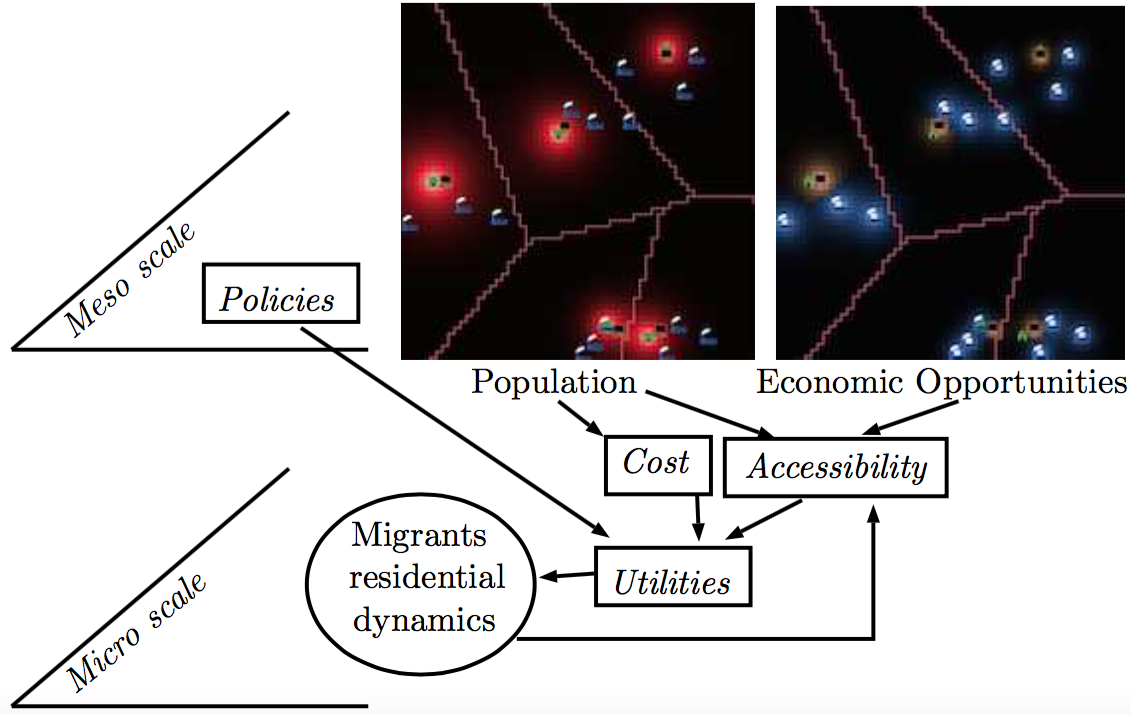
\includegraphics[width=\textwidth]{figures/model}
\caption{Multi-scale schema of processes included in the model}
\label{fig:model}
\end{figure}
%%%%%%%%%%%%%%%


\subsection{Model Description}

\paragraph{Setup}

The world consists in a lattice of $1 \leq i \leq N$ cells, characterized by their population $P_i(t)$ and an economic structure $E_i^{(c)}(t)$ which consists in abstract variables representing potential number of jobs stratified by socio-economic classes $c$. The associated effective number of workers is denoted by $W_i^{(c)}(t)$. For the sake of simplicity, we assume a discrete number of classes. At initial time, the variables are initialized either following a synthetic data generation process (see below), or from real geographical data (abstracted and simplified to fit our context). Cells are grouped into $1\leq k\leq K$ administrative cities that corresponding to the various centers of the MCR, on which aggregated population $\tilde{P}_k(t)$ and corresponding economic variables ($\tilde{E}_k^{c}(t)$) can be computed.

\paragraph{Agents}

An agent is a household of migrants, whose residence and job are located in cells (that can be different). Socio-economic structure of the population is captured by the distribution of wealth $g(w)$, which are then stratified into categories. At a given time, the utility difference between not moving and moving to cell $j$ from cell $i$, for a category $c$ is given by

\[
\Delta U_{i,j}^{(c)}(t) = \frac{Z_j^{(c)}- Z_i^{(c)}}{Z_0} + \frac{C_i^{(c)}- C_j^{(c)}}{C_0} - u_i^{(c)} - h_j^{(c)}
\]

where $Z_i^{(c)}$ is generalized accessibility given by $Z_i^{(c)} = P_i \cdot \sum_k \left[E_k^{(c)}-W_k^{(c)}\right]\cdot \exp{\left(\frac{-d_{ij}}{d_0}\right)}$, with $d_{ij}$ effective travel distance (in public transportation ; \textit{point to be clarified : for higher classes, car may be an option}) and $d_0$ commuting characteristic distance ; $C_i^{(c)}$ is the cost of life which is a function of cell and city variables, that will be taken as $C_i^{(c)} \propto P_i^{\alpha_0}\cdot  \tilde{P}_i^{\alpha_1}\cdot$ ; $u_i^{(c)}$ a baseline aversion to move and $h_j^{(c)}$ an exogenous variable corresponding to regulation policies ; $Z_0$ and $C_0$ dimensioning parameters.

\paragraph{Temporal Evolution}

At each time step, the system evolves sequentially according to the following rules :

\begin{enumerate}
\item Cities mesoscopic variables $\tilde{P}_k(t)$ and $\tilde{E}_k^{c}(t)$ are deterministically updated. Population follows the very simple assumption of the expectancy of a Gibrat's law, i.e. $\tilde{P}_k(t)= g_k \cdot \tilde{P}_k(t-1)$. Economy follows a scaling law of population: $\tilde{E}_k^{(c)}(t) = E_k^{(c,0)}\cdot \left(\frac{\tilde{P}_k(t)}{P_0}\right)^{\gamma_k^{(c)}}$.

\item Patches variables are updated conditionally to the new aggregated values. For population, we adapt the aggregation-diffusion process detailed in~\cite{raimbault2016calibration}: a density ceil is introduced and diffusion is replaced by spatial noise\footnote{formally, let $\Delta \tilde{P}_k(t) = \tilde{P}_k(t) - \tilde{P}_k(t-1)$}.

%\textit{Using a simple urban growth model of aggregation, deterministic for population and a bit more random for jobs ; still to be clarified}.

\item A number of new migrants, proportional to Gibrat growth rate, enter the region. They lean on social network (关系,guanxi) 
to first settle in the city and agglomerate following a preferential attachment by place of origin.
\item Migration occur following a discrete choice dynamics : the probability to move to cell $j$ is given by

\[
\Pb{i\rightarrow j | c} = \frac{\exp{\left(\beta\cdot U_j^{(c)}\right)}}{\sum_k \exp{\left(\beta\cdot U_k^{(c)}\right)}+\exp{\left(U_{stay,i}^{(c)}\right)}}
\]

what simplifies into a reduced form, with $\beta' = \frac{\beta}{Z_0}$, $\gamma = \frac{Z_0}{C_0}$ and $\tilde{u},\tilde{h}$ accordingly rescaled variables, using the above utility expression :

\[
\Pb{i\rightarrow j | c} = \frac{\exp{\left(\beta'\cdot \left[\Delta Z_{i,j}^{(c)} - \Delta C_{i,j}^{(c)} - \tilde{u}_i^{(c)} - \tilde{h}_j^{(c)} \right] \right)}}{1 + \sum_k {\exp{\left(\beta'\cdot \left[\Delta Z_{i,k}^{(c)} - \Delta C_{i,k}^{(c)} - \tilde{h}_k^{(c)} \right] \right)} - N\cdot \tilde{u}_i^{(c)}}}
\]

Residential movement is drawn randomly according to these probabilities, and jobs are chosen around new residence following an exponentially decreasing probability.

\item Migrants update their wealth and eventually economic category

\end{enumerate}


\paragraph{Indicators}

\begin{itemize}
\item Total migrants wealth gain
\item Total migrants social mobility
\item \todo{segregation ?}
\end{itemize}


\paragraph{Synthetic Data Generation}



\textit{TBW}



%%%%%%%%%%%%%%%%%%%%
\section{Results}



\todo{
Next steps :
\begin{itemize}
\item Full exploration on synthetic data : model behavior
\item Stylization and scenarization of real DPR configuration, model behavior on real and hybrid configurations
\item Targeted experience plans (e.g. : role of economic diversity, influence of state regulation)
\item Iterative further construction/multi-modeling (e.g. generations)
\end{itemize}
Expected Results :
\begin{itemize}
\item Impact of processes linked to migrants diversities on emergent dynamics
\item Explore or unveil state strategies (through regulations or companies control)
\end{itemize}
}



\paragraph{Model Validation}

\begin{itemize}
\item Internal validation : statistical consistence ; system trajectories ; path-dependency.
\item External validation : stylized facts from synthetic data exploration ?
\end{itemize}


%%%%%%%%%%%%%%%%
\begin{figure}
\centering
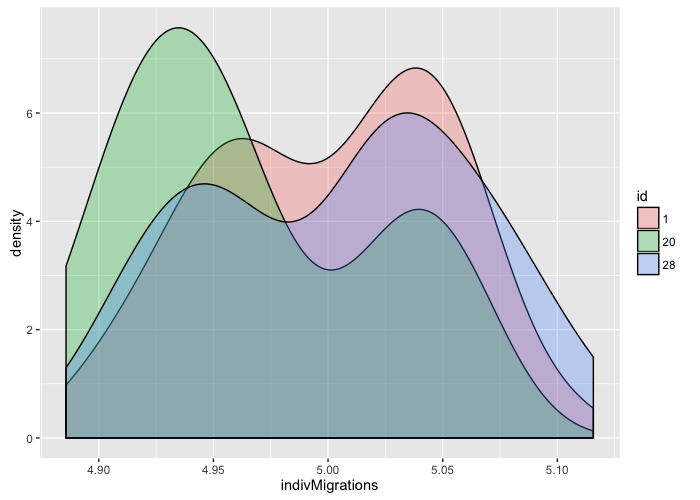
\includegraphics[width=0.45\textwidth]{figures/hist_indiv}
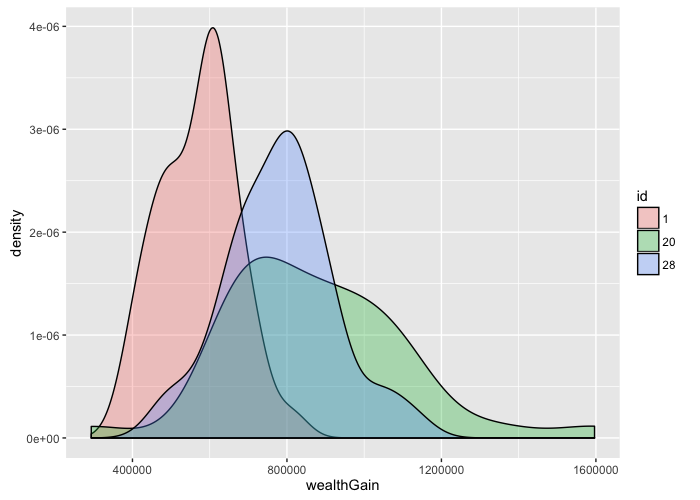
\includegraphics[width=0.45\textwidth]{figures/hist_wealthGain}
\caption{Statistical distributions of number of individual migrations and wealth gain over ? runs, for some example parameter points}
\label{fig:statistical-valid}
\end{figure}
%%%%%%%%%%%%%%%%



%%%%%%%%%%%%%%%%
\begin{figure}
\centering
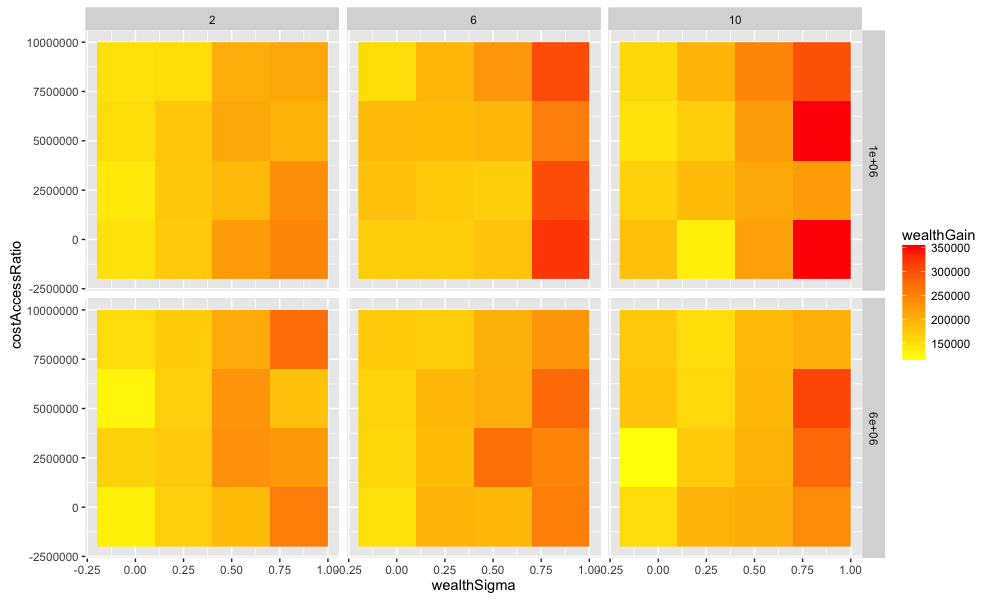
\includegraphics[width=\textwidth]{figures/wealthGain}\\
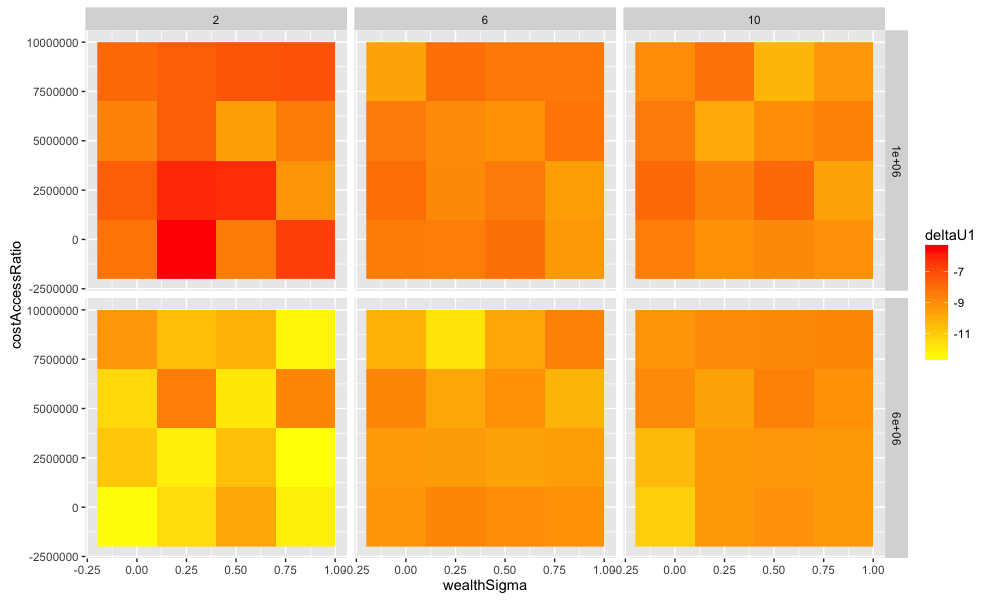
\includegraphics[width=\textwidth]{figures/deltaU1}
\caption{Phase diagrams in 4 dimensional parameter space, over ? runs, for wealth gain and $\Delta U_1$}
\label{fig:statistical-valid}
\end{figure}
%%%%%%%%%%%%%%%%





\paragraph{Application}

\textit{Stylize Pearl River Delta configuration}

\paragraph{Experience Plan} \textit{concrete qualitative questions that can be asked to the model, e.g. :
\begin{itemize}
\item what is the impact of varying wealth distribution shape and width on system dynamics/migrant trajectories ?
\item what is the impact of various spatial distribution of $h_j^{(c)}$, i.e. different government policies ?
\item Comparison with and without Hong-Kong and Macao
\item \ldots
\end{itemize}
}



%%%%%%%%%%%%%%%%%%%%
%% Biblio
%%%%%%%%%%%%%%%%%%%%

\bibliographystyle{apalike}
\bibliography{biblio}


\end{document}
